\documentclass[a4paper,10pt]{report}
\usepackage[utf8x]{inputenc}
\usepackage[french]{babel}
\usepackage[T1]{fontenc}
\usepackage{latexsym}
  \usepackage{algorithm,algorithmic}
\usepackage{graphicx}
\usepackage{amssymb, amsmath}

%%% francisation des algorithmes
\renewcommand{\algorithmicrequire} {\textbf{\textsc{Entrées:}}}
\renewcommand{\algorithmicensure}  {\textbf{\textsc{Sorties:}}}
\renewcommand{\algorithmicwhile}   {\textbf{tantque}}
\renewcommand{\algorithmicdo}      {\textbf{faire}}
\renewcommand{\algorithmicendwhile}{\textbf{fin tantque}}
\renewcommand{\algorithmicend}     {\textbf{fin}}
\renewcommand{\algorithmicif}      {\textbf{si}}
\renewcommand{\algorithmicendif}   {\textbf{finsi}}
\renewcommand{\algorithmicelse}    {\textbf{sinon}}
\renewcommand{\algorithmicthen}    {\textbf{alors}}
\renewcommand{\algorithmicfor}     {\textbf{pour}}
\renewcommand{\algorithmicforall}  {\textbf{pour tout}}
\renewcommand{\algorithmicdo}      {\textbf{faire}}
\renewcommand{\algorithmicendfor}  {\textbf{fin pour}}
\renewcommand{\algorithmicloop}    {\textbf{boucler}}
\renewcommand{\algorithmicendloop} {\textbf{fin boucle}}
\renewcommand{\algorithmicrepeat}  {\textbf{répéter}}
\renewcommand{\algorithmicuntil}   {\textbf{jusqu'à}}

\newcommand{\Fp}{\mathbb{F}_p}
\newcommand{\Pp}{\mathbb{P}_1(\Fp)}

% Title Page
\title{Algorithme rho de pollard}
\author{TAFFOREAU Nicolas}


% -----------------------------------------
% organisation a revoir 
% -----------------------------------------

\begin{document}
\maketitle
\tableofcontents
\chapter{Introduction}

\section{Rappel sur les courbes elliptique}
% 2 pages

    Soit un corps $\Fp$ ($p > 3$ premier), et soit $a, b \in \Fp$
tels que $4 a^3 + 27 b^2 \ne 0$.
La courbe elliptique $E/\Fp: Y^2 = X^3 + aX + b$ est définie par l'ensemble
des points $(x:y:z)\in \Pp$ tel que soit satifaite l'équation 
$$ z y^2 = x^3 + a x z^2 + b z^3.$$

  Si z = 0 alors x = 0 et donc on obtient $(0,k,0)$ qui est un élément inversible donc peut être réduit à $(0,1,0)$, ce point scpécifique est appelé le point à l'infini.

  L'ensemble de ces points forment un groupe abélien avec comme zero, le point à l'infini et possède un loi de groupe.
  Soit P, $Q \in F$, $ P = (x_1,y_1)$, $Q = (x_2,y_2)$ alors $P+Q = (x_3,y_3)$ tel que 
    \begin{center}
      $x_3 = \mu^2 -x_1 - x_2$, $y_3 = \mu(x_1-x_3)$
    \end{center}
    \begin{center}
      $\mu = \frac{y_2 - y_1}{x_2 - x_1}$ si $P \ne Q$
    \end{center}
    \begin{center}
      $\mu = \frac{3*x_1^2 + a}{2*y_1}$ si $P = Q$
    \end{center}


Une propriété importante sur les courbes elliptiques est le calcule de l'inverse d'un point pour la loi d'addition sur Fp. Si $P = (x_1,y_1)$ alors $-P = (x_1,-y_1)$.

On peut avoir aussi la courbe définit sur $Fq$ avec $q = p^n$, certaines propriétés sont un peut différentes.
Pour une courbe elliptique sur $Fq$, si $P = (x_1,y_1)$ alors $-P = (x_1,y_1+x_1)$.

\section{Algorithme rho de Pollard}

\subsection{Dans un groupe du type Fp}

Dans un groupe du type Fp, Pollard a choisit comme marche aléatoire un fonction qui ne tient compte que de l'élément précédent.\\

\begin{itemize}
\item{marche aléatoire}\\
{
$ f(x) = x*P$ si $x \in [0;p/3[$\\
$ f(x) = x*x$ si $x \in [p/3;2p/3[$\\
$ f(x) = x*Q$ si $x \in [2p/3;p[$\\
}
\end{itemize}

En utilisant cette marche aléatoire il en a deduit un algorithme en se basant sur l'algorithme de floyd pour trouver rapidement la longueur d'un cycle.

Ici P est un generateur du groupe et Q est l'élément dont on veut connaitre le logarithme en base P.

{
 \begin{algorithm}
 \caption{rho pollard}
 \begin{algorithmic}
  \REQUIRE n,P,Q
  \ENSURE x tel que Q = $P^x$ mod n
    \STATE $[W1,a,b] \leftarrow$ combinaision aleatoire de $P$ et $Q$
    \STATE $[W2,a',b'] \leftarrow$  marche aléatoire à partir de $W1$
	\STATE ($W2 = P^{a'} + Q^{b'}$)
    \WHILE{$ W1 \ne W2$}
      \STATE $[W1,a,b] \leftarrow$ marche aléatoire à partir de $W1$
      \STATE $[W2,a',b'] \leftarrow$ marche aléatoire à partir de $W2$
      \STATE $[W2,a',b'] \leftarrow$ marche aléatoire à partir de $W2$
    \ENDWHILE
  \IF{ $b-b' = 0$ $modulo$ $n$}
    \STATE echec pour trouver le logarithme discret
  \ELSE
    \STATE $ x = \frac{a'-a}{b-b'}$ $modulo$ $n$
  \ENDIF
 
 \end{algorithmic}
 \end{algorithm}
 }


L'algorithme rho de pollard est identique sur les courbes elliptiques sauf que l'on se place dans un cas plus générale,
seul la marche aléatoire change. On applique des additions et de scalaires sur la courbe elliptique au lieu de la multiplication modulaire et du carré modulaire.

Le nom de cette algorithme est dû à la forme que prend la suite aléatoire, on a d'abord un pré-cycle puis le cycle.

\begin{center}
 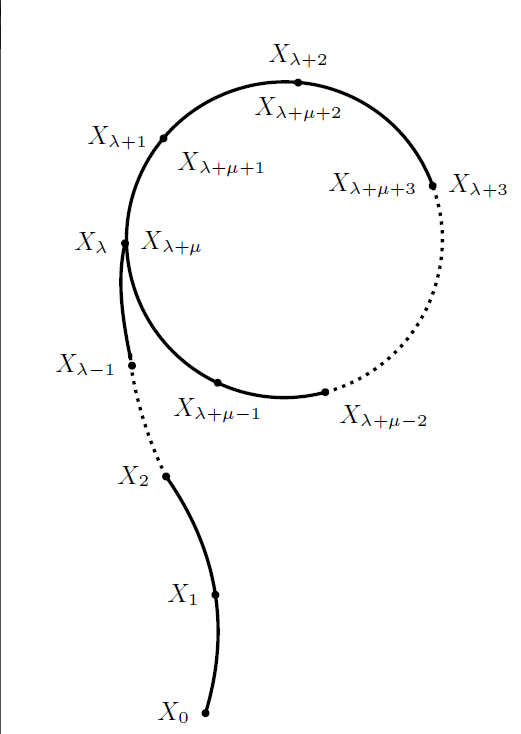
\includegraphics[width=4cm]{dessin_rho_pollard_bon.png}
\end{center}

\subsection{Paradoxe des Anniversaires}
L'algorithme rho de pollard est basé sur le paradoxe des anniversaires.

 Dans un groupe fini si on prend des éléments de façon aléatoire,
il faut en moyenne tirer $\sqrt{n}$ éléments pour obtenir un élément que l'on à déjà tiré, ou n est le nombre d'élément de notre ensemble.

La formule générale pour obtenir une probabilité d'intersection ($I(n)$) est 1-$p(n)$ où $p(n)$ est la probabilité d'avoir aucune intersetion sur n tirages avec remise dans un groupe de $m$ éléments
\begin{center}
    $p(n) = \frac{m!}{(m - n)!}*\frac{1}{m^n}$
    $I(n) = 1 - \frac{m!}{(m - n)!}*\frac{1}{m^n}$
\end{center}




\subsection{algorithme de floyd}

Il existe différent moyen pour trouver une collision dans un cycle, le meilleur algorithme pour en trouver
une est l'agorithme de floyd qui permet de calculer de façon très rapide la longueur d'un cycle en se basant sur des collisions.
La propriété qu'il a énoncé est que dans un groupe cyclyque si on a une marche aléatoire cyclique, alors au lieu de stocké chaque 
éléments et de vérifier si il n'est pas dans la liste. il calcule l'élément i et 2i de cette marche aléatoire juqu'à avoir une 
collision.

exemple sur le groupe Z/17Z, avec la mache aléatoire $f(x) = x^x + 1 mod 17$.
si x = 1 -> 2 -> 5 -> 9 -> 13 -> 16 -> 0 -> 1
donc $a_1 = 1, a_2 = 2, a_3 = 5 .....$
// mauvais choix puissance de 2

\chapter{verification de la comlpexité de l'algorithme rho de pollard}

L'algorithme rho de pollard est estimé, d'après le papier de Stephen D. Miller et Ramarathnam Venkatesan, \textit{Spectral Analysis of Pollard Rho Collisions} en $O(\sqrt{n}(\log{n})^3)$. 
Quand n temps vers l'infini c'est le logarithme est négligeable par rapport à la racine de n. On peut donc approximé cette complexité en $O(\sqrt{n})$.

Pour montrer que l'algorithme est bien dans une complexité s'approchant de la racine de n, j'ai effectué des tests de résolutions du logarithme discret avec la methode initiale
de Pollard. La marche aléatoire que j'ai pris est définie par : \\
\begin{itemize}
 \item {marche aléatoire}\\
  $ f(W) = W \oplus P$ si $x = 0$ $modulo$ $3$ \\
  $ f(W) = 2*W$ si $x = 1$ $modulo$ $3$ \\
  $ f(W) = W \oplus Q$ si $x = 2$  $modulo$ $3$ \\
  $ W = [x,y] $ \\
\end{itemize}

Ici le $\oplus$ est l'addition sur la courbe elliptique et le $2*W$ est l'oppération de doublement sur la courbe elliptique.

Pour obtenir des valeurs facile pour faire une comparaison, il est plus simple de changer l'échelle et de regarder avec une echelle logarithmique.\\
\begin{center}
 $\sqrt{n} = n^{\frac{1}{2}}$
 Si $n=2^x$ alors en échelle logarithimque (base 2) $\log{n} = x$ et $\log{\sqrt{n}} = \frac{x}{2}$
\end{center}

Donc si on fait une régression linéaire des différents valeurs trouvées, on devrait obtenir une droite avec un coefficient de 0,5.

\begin{center}
 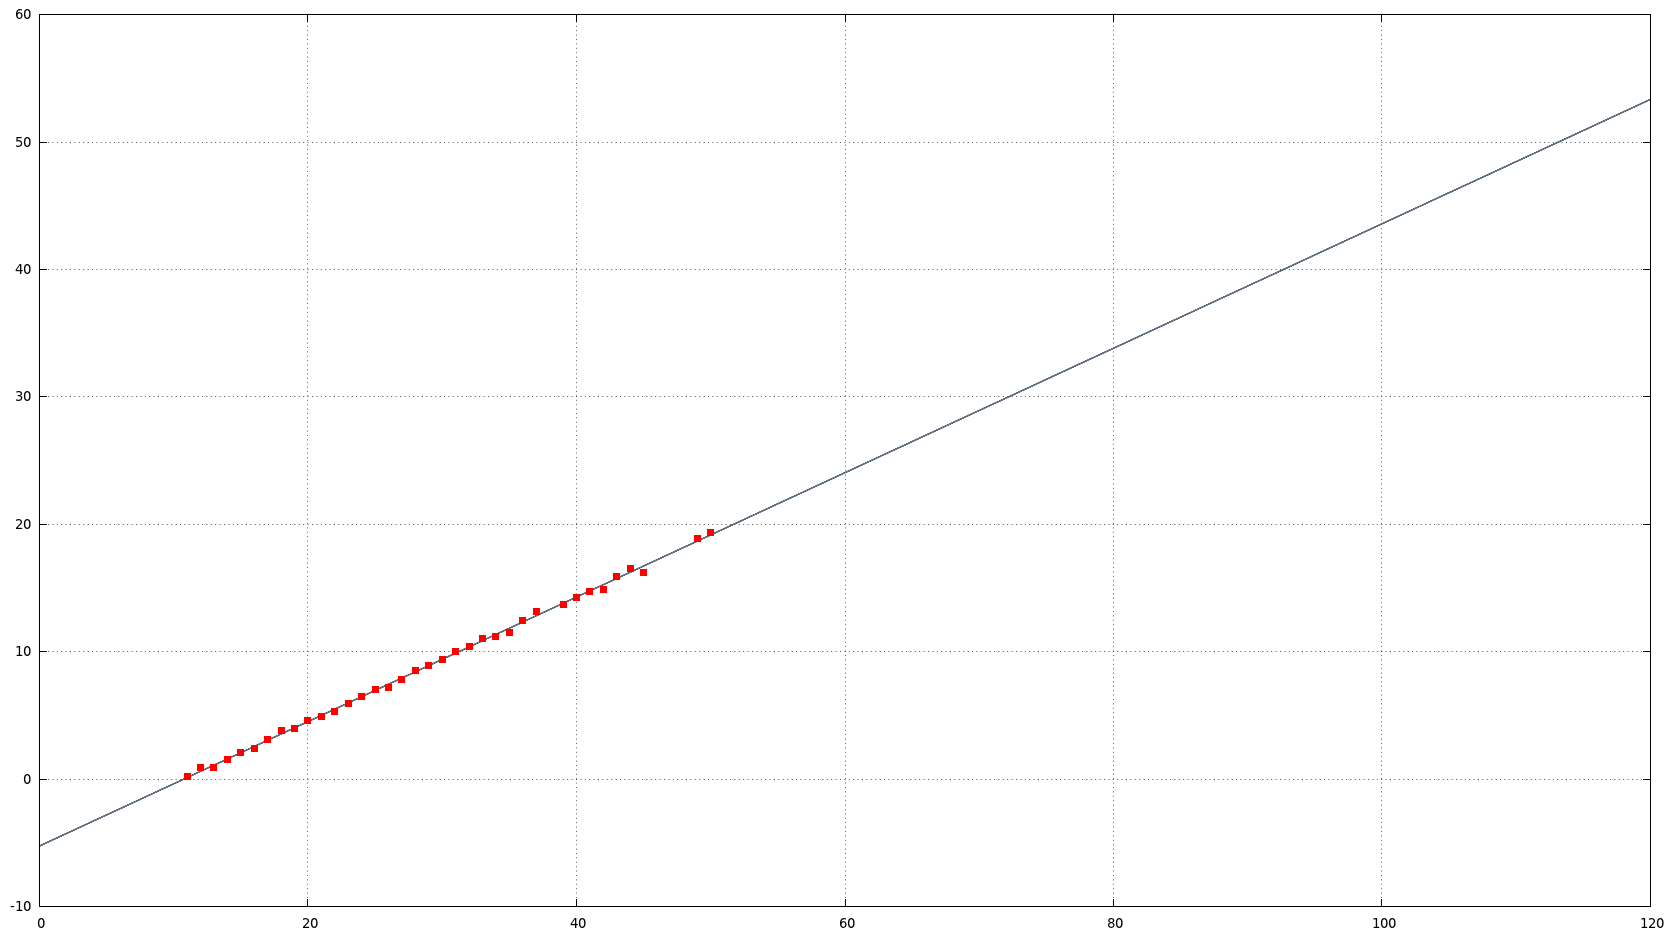
\includegraphics[width = 15cm]{regresion_rho_normal_bon.png}
\end{center}


% \begin{center}
% \begin{verbatim}
%  Mon Feb 20 14:32:17 2012
% 
% 
% FIT:    data read from './temp_moyen_courbe_normal.txt'
%         format = z
%         #datapoints = 36
%         residuals are weighted equally (unit weight)
% 
% function used for fitting: f(x)
% fitted parameters initialized with current variable values
% 
% 
% 
%  Iteration 0
%  WSSR        : 17090.3           delta(WSSR)/WSSR   : 0
%  delta(WSSR) : 0                 limit for stopping : 1e-05
%  lambda	  : 21.8908
% 
% initial set of free parameter values
% 
% a               = 1
% b               = 1
% 
% After 5 iterations the fit converged.
% final sum of squares of residuals : 1.32396
% rel. change during last iteration : -4.13064e-11
% 
% degrees of freedom    (FIT_NDF)                        : 34
% rms of residuals      (FIT_STDFIT) = sqrt(WSSR/ndf)    : 0.197332
% variance of residuals (reduced chisquare) = WSSR/ndf   : 0.0389399
% 
% Final set of parameters            Asymptotic Standard Error
% =======================            ==========================
% 
% a               = 0.48823          +/- 0.002987     (0.6118%)
% b               = -5.24743         +/- 0.09242      (1.761%)
% 
% 
% correlation matrix of the fit parameters:
% 
%                a      b      
% a               1.000 
% b              -0.935  1.000 
% \end{verbatim}
% \end{center}

\chapter{Negation map}

\section{methode general}

Sur une courbe elliptique sur Fp l'inverse de P = (x,y,z), simplifié à (x,y) est -P = (x,-y). le but de cette méthode est de reduire le groupe de moitier,
donc de faire une recherche de log discret dans <P>/<H>. On obtient donc une relation du type $\pm[a]P \pm[b]Q = \pm[a']P \pm[b']Q$. Il nous suffit donc de retrouver exactement 
la relation avec les bon signe pour retrouver le logarithme discret.

Premier problème on retombe très rapidement sur le meme point avec les meme scalaires, si on évite ses point et que l'on continue la boucle, elle continue indéfiniment.
En plaçant des prints sur l'égalité et un compteur générale de boucle, on remarque que comme décrit dans l'article on a l'apparition de cycle court de longueur 2.

La méthode décrite dans l'article \" ...\" nous dis de garder en mémoire quelque points de la marche aléatoire, puis de faire un comparaison pour detecter si on entre dans un cycle
longueur 2, cette comparaison s'effectue entre le terme que l'on vient de calculer et celui qui était deux crant avant.
S'ils sont différents alors on continue la marche comme elle était, mais s'ils sont identiques alors le point suivant est $2*min(W_{-1},W_{-2})$ où le min est le minimun lexicographique et
la multiplication par 2 est l'oppération de doublement sur la courbe elliptique.

Après enlèvement de ces cycle infructueux de taille 2, on retombe dans des cycles de taille 4.

\section{cycle infructueux}

apppartition très fréquente de cycle de taille 2 n'important pas d'information sur le log discret on les elimine donc en ......

\chapter{random walk}

Dans l'article de \textit{Bernstein}, il est fait référence au fait que \textit{Pollard} n'utilisait que trois groupes pour faire sa marche aléatoire, 
alors que Teske dans son papier \textit{On random walks for pollard's rho method} nous dis qu'il est beaucoup plus efficase d'utilisé plus de groupe 
pour faire une marche aléatoire.

Dans son article \textit{Teske} introduit un indice L :
\begin{center}
 $ L = \frac{nombre d'iteration avant de trouver une collision}{\sqrt(|G|)} $
\end{center}

J'ai donc implémenté une fonction qui au lieu d'utiliser une marche aléatoire sur 3 groupe en faisant soit $+P$, $+Q$, ou un doublement,
utilise r groupe où on ajoute à notre élément un élément spécifique du groupe. Ces différents éléments sont au préalable tiré aléatoirement.
Je fais donc une marche additive, pour chaque $W_i$ je lui ajoute un $R_j$ où j est un hash de i. On a donc la formule suivante : 
$ W_{i+1} = W_{i} + R_{h(i)} $.

Pour connaître à quel groupe appartient l'élément, je regarde sa première composante modulo r.

\textit{Teske} après expérimentation trouve que pour la valeur $r >= 20$ ont atteint un bien meilleur ratio pour l'indice L.

En refaisant les test j'obtient une valeurs identique, au dela de 20 on fait beaucoup de precalcule pour peu d'amélioration.


point important : plus trop une marche alléatoire pour 3 groupes donc plus pour r groupes r > 19.

\chapter{endomorphisme}
 
 ????

\chapter{parrallelisation}

pour parralelisé le log discret on definie une règle pour avoir des point remarquable (tel que ....) 
a chaque fois que l'on a après une marche un point remarquable on le transmet a un serveur central ainsi que les donné de départ
quand on  a deux intersection de point remarquable on a une collision.

\section{choix des points remarquables}

Mon choix est de prendre des point dont la première variable (x) possède un certain nombre de bit de poids faible à zeros.
J'ai fait différents tests : prendre $log(p)/log(2)/3$ ou $log(p)/log(2)/4$ appartition de pallier entre le nombre de point remarquable et le cardinal du groupe.
groupe de 3 avec même poucentage d'éléments remarquables dans le groupe.

\begin{verbatim}
 ? for( p = 15,30, n = prem_n_bit(p); E = courbe_ell_Fp(n); P = random(E); w = proba_remarquable(E,P);o = ellorder(E,P)+0.1; print(w/o));
0.0340
0.0312
0.0307
0.0155
0.0155
0.0157
0.0079
0.0078
0.0078
0.0039
0.0039
0.0039
0.0020
0.0020
0.0020

\end{verbatim}



calcule à faire en se basant sur le paradoxe des anniversaire pour tomber sur un point remarquable et pour avoir deux points remarquables identiques.

detail de l'algorithme.

\chapter{bibliograpie}
Edlyn Teske, on a random walks for pollard's rho method.

Daniel J. Bernstein, Tanja Lange, Peter Schwabe, On the correct use of negationmap in the pollard's rho method.

John M.Pollard, monte carlo method for index computation mod p.

Wikipedia.
\end{document}          
